\documentclass[11pt]{article}
\usepackage[margin=1.15in]{geometry}
\usepackage{amsmath,amssymb,amsthm}
\usepackage{booktabs}
\usepackage{graphicx}
\usepackage{microtype}
\usepackage[authoryear,round]{natbib}
\usepackage[colorlinks=true,linkcolor=black,citecolor=black,urlcolor=black]{hyperref}
\usepackage{setspace}
\onehalfspacing

\newtheorem{proposition}{Proposition}
\newtheorem{remark}{Remark}
\theoremstyle{definition}
\newtheorem{definition}{Definition}

\newcommand{\E}{\mathbb{E}}
\newcommand{\Var}{\operatorname{Var}}
\newcommand{\N}{\mathcal{N}}

\title{Where the Averaging Goes\\[4pt]
\large Endpoint Regression, Local Velocity Fields, and the Last Euler Step}
\author{Flyxion\\Independent Researcher}
\date{October 2026}

\begin{document}
\maketitle

\begin{abstract}
\noindent
A common summary of why generative models help with multimodal targets is that regression averages and generation does not. This summary is half right, and the wrong half causes errors. A squared-error regressor outputs a conditional mean, and when the target is bimodal the mean can lie where no data exist. A flow-matching model is also trained by squared-error regression, and its velocity field is also a conditional mean. The difference is the object being averaged and the information the average is conditioned on. This essay works out the difference exactly in a two-component Gaussian mixture, where every quantity has a closed form. It shows that a one-step flow reproduces the regression mean exactly, that the exact field defers and localizes the averaging rather than abolishing it, that the interval over which the two modes become distinguishable has a simple analytic location, and that the numerical integrator reintroduces endpoint averaging at a scale set by the final step size relative to the within-mode spread. A simulation with $2\times 10^5$ samples agrees with each statement to within Monte Carlo error. The conclusions are stated for the exact field in one dimension. What they imply for learned networks and for any particular system is limited, and the limits are listed.
\end{abstract}

\section{Two averages}

Consider a decision problem with two good answers. A scene contains two doorways, and the useful anchor for exploration is the center of either one. A regressor trained with squared error on examples that split evenly between the doorways converges to the average of the two answers, which is the wall between them. The point is familiar, and it is the stated motivation for a large family of generative approaches to decision making: replace the regressor with a model that samples, and the average is no longer taken.

That last clause is where the summary needs care. A flow-matching model is trained by minimizing a squared error as well. Its target is the displacement $x_1-x_0$ between a noise sample and a data sample, and the minimizer is a conditional expectation of that displacement given the current position and time \citep{lipman2023}. An expectation is an average. The statement ``generation does not average'' cannot be literally true of this training objective, and it is not. What is true is narrower, and it can be stated precisely.

\begin{quote}
The regressor averages over \emph{endpoints}, conditioned on the observation alone. The flow field averages over \emph{velocities}, conditioned on the observation, the current position and the current time. Conditioning on position and time lets the average become less and less ambiguous as paths separate, and the sampler follows the field through that separation.
\end{quote}

The essay develops this in a setting small enough to solve. Section~2 fixes a two-mode Gaussian target. Section~3 shows that a flow integrated in one step is the regression mean. Section~4 describes the exact field and where its ambiguity sits in time. Section~5 treats the numerical integrator, whose last step is itself an average. Section~6 reports what a simulation shows. Section~7 connects the results to a recent exploration paper that motivates multi-anchor sampling with the endpoint-averaging argument \citep{li2026}, and Section~8 lists four common misreadings that the analysis corrects. Section~9 states limits.

\section{A two-mode model with closed forms}

Let the data variable $x_1$ be a symmetric mixture of two Gaussians,
\[
x_1\sim \tfrac12\N(-a,\sigma^2)+\tfrac12\N(a,\sigma^2),
\]
and let the source be $x_0\sim\N(0,1)$, independent of $x_1$. The linear interpolation path is $x_s=(1-s)x_0+s x_1$ for $s\in[0,1]$, and the conditional flow-matching target is $u=x_1-x_0$. The regression minimizer is
\[
v^\ast(x,s)=\E[x_1-x_0\mid x_s=x]=\frac{m(x,s)-x}{1-s},\qquad m(x,s)=\E[x_1\mid x_s=x].
\]
The second equality holds for $s<1$ because $x_0=(x-s x_1)/(1-s)$ on the event $x_s=x$. At $s=1$ the formula is undefined, and the field is determined only as a limit.

In this model everything is Gaussian given the component. Write $k\in\{-,+\}$ for the component and $\tau^2(s)=s^2\sigma^2+(1-s)^2$. Given $k$, the variable $x_s$ is $\N(s\mu_k,\tau^2)$ with $\mu_\pm=\pm a$, and
\[
x_1\mid x_s=x,\,k\ \sim\ \N\!\Big(\mu_k+\frac{s\sigma^2}{\tau^2}(x-s\mu_k),\ \frac{\sigma^2(1-s)^2}{\tau^2}\Big).
\]
The posterior weight of the upper component is the logistic function
\[
w_+(x,s)=\Big(1+\exp\!\big(-2as\,x/\tau^2(s)\big)\Big)^{-1},\qquad w_-=1-w_+ .
\]
These three facts determine $m$, the field $v^\ast$, the posterior variance of $x_1$, and the training-loss floor
\[
L^\ast(s)=\E\big[\Var(x_1\mid x_s)\big]/(1-s)^2 .
\]
Appendix~A collects the derivations. The parameters used throughout are $a=1$ and $\sigma=0.1$.

\section{A one-step flow is the regression mean}

The first statement is exact and does not depend on the mixture.

\begin{proposition}
Let $x_0$ be independent of $x_1$. If the exact field $v^\ast$ is integrated with a single Euler step from $s=0$ to $s=1$, the output is the constant $\E[x_1]$ for every starting point $x_0$.
\end{proposition}

\begin{proof}
At $s=0$ the observation $x_{0}=x_s$ carries no information about $x_1$, so $m(x,0)=\E[x_1]$ and $v^\ast(x,0)=\E[x_1]-x$. One Euler step of length one gives $x_0+v^\ast(x_0,0)=\E[x_1]$. \qedhere
\end{proof}

In the symmetric mixture, $\E[x_1]=0$, and every sample lands at the midpoint between the modes. The output has no mass within $a/2$ of either mode, and its 1-Wasserstein distance to the target is $\E|x_1|=\sigma\sqrt{2/\pi}\,e^{-a^2/2\sigma^2}+a\,[1-2\Phi(-a/\sigma)]$, which equals $a$ to the precision reported here because $a/\sigma=10$ but is not exactly $a$ for a target with Gaussian tails. The sampler has not escaped the average. It has been run for so few steps that it implements the average.

This observation locates the benefit of the generative formulation more precisely than the slogan does. The benefit is not a property of the loss. It is a property of how many times, and at what positions, the field is consulted.

\section{The exact field defers and localizes the average}

\subsection{The first step still averages}

At small $s$ the paths from the two components overlap almost entirely, and the field at every position points toward the global mean. The average that the regressor takes at the first decision is also taken by the field at the first step. What changes along the trajectory is the set of paths that pass through the current position.

\subsection{When the paths separate}

Given component $k$, the position $x_s$ has mean $s\mu_k$ and spread $\tau(s)$. The two components are separated in units of spread by
\[
d(s)=\frac{a s}{\tau(s)} .
\]
Because the two conditional laws are Gaussian with equal variance and equal prior weight, the Bayes error for identifying the component from $x_s$ is exactly $\Phi(-d(s))$. The log-odds $\log(w_+/w_-)$ is normal with mean $2d^2$ and variance $4d^2$ when the true component is $+$.

Setting $d(s)=1$ gives $a^2s^2-s^2\sigma^2=(1-s)^2$, that is $s_c=1/(1+\sqrt{a^2-\sigma^2})$ for $a>\sigma$, which is $0.5013$ here and is approximately $1/(1+a)$ for small $\sigma$. The same value marks the point at which the symmetric marginal $p_s$ changes from one mode to two, since an equal mixture of two Gaussians of common spread $\tau$ is bimodal exactly when the means are more than $2\tau$ apart. It is an analytic threshold for distinguishability, not a time after which averaging ceases to matter. The Bayes errors for $s=0.1,0.3,0.5,0.7,0.9$ are $0.456,\,0.334,\,0.160,\,0.012$ and $<10^{-3}$. A separate statistic, the mean posterior entropy of the mode, first falls below half a bit at $s=0.52$ on a time grid of spacing $0.02$. The two indicators are related measures of increasing distinguishability and are not a single commitment time.

The consequence is that the field's ambiguity is not spread evenly over time. Well before $s_c$ the mode is poorly determined by the position, and well after it the field points toward the correct mode with high probability. A position left of the midpoint after $s_c$ is carried toward $-a$, and a position right of it toward $+a$. The trajectories in Figure~1 show this, with paths that begin near each other on opposite sides of the midpoint diverging in the interval around $s_c$.

\begin{figure}[t]
\centering
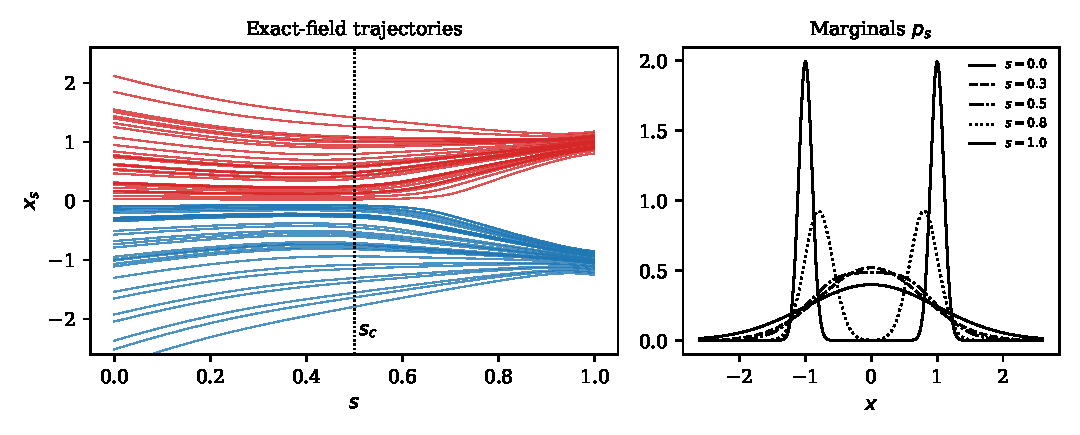
\includegraphics[width=\textwidth]{fig_traj.pdf}
\caption{Exact-field trajectories for sixty noise samples (left) and the marginal densities $p_s$ at five times (right). Paths from the two sides of the midpoint separate around $s_c\approx0.5$. Colors mark the mode reached at $s=1$.}
\end{figure}

\subsection{What the paths do not do}

A frequent worry is that the field averages incompatible velocities at crossing points and therefore sends samples to the middle. For the exact field this does not happen in the way imagined. The field is a single-valued function of position and time, and trajectories of an ordinary differential equation with a smooth single-valued right-hand side do not cross. The velocities of conditional paths \emph{do} cross, and the field is their average at the crossing, which is precisely why the integral curves of the average remain separate. The average is what removes the crossing. The sampler then reproduces the marginals $p_s$ because the field and the marginal path satisfy the same continuity equation \citep{lipman2023}.

\subsection{Where the local gradients are large}

Uniqueness of the integral curves does not mean the field is gentle along them. At the midpoint $x=0$ the derivative of the field in $x$ has the closed form
\[
\partial_x v^\ast(0,s)=\frac{1}{1-s}\left[\frac{s\sigma^2}{\tau^2}+\frac{a^2 s(1-s)^2}{\tau^4}-1\right].
\]
For $\sigma=0.1$ and $a=1$ this reaches a maximum of about $361$ at $s=0.942$, and the leading behavior for small $1-s$ and $\sigma$ is of order $a^2/\sigma^3$, attained near $1-s\approx\sigma/\sqrt3$. A large positive derivative means strong local expansion of nearby trajectories, so small perturbations of position are magnified there. It does not by itself establish stiffness in the numerical-analysis sense, and it does not establish how errors in a learned field propagate. For $\sigma\to0$ the maximum diverges, the one-dimensional counterpart of the fact that the exact field for a discrete target is not Lipschitz up to $s=1$.

\subsection{The loss floor}

The best achievable training loss at time $s$ is $L^\ast(s)$. In the model it equals $1.05$ at $s=0.02$, rises to a maximum of $1.91$ near $s=0.42$, and falls to $0.45$ at $s=0.7$, $0.55$ at $s=0.9$, and $1.0$ at $s=0.98$. Two sources of irreducible error are mixed here. Near the middle of the path it is mostly the ambiguity about which mode the sample belongs to. Near the end, once the endpoint is almost determined by $x_s$, the remaining uncertainty is in the velocity target itself: $u=x_1-x_0$, and conditioning on $x_1$ leaves $\Var(u\mid x_1)=\Var(x_0)=1$ because the source draw is independent of the endpoint. The floor therefore tends to $1$ as $s\to1$ for a reason unrelated to mode ambiguity. A floor that is high at late flow time does not by itself indicate unresolved mode ambiguity, and flow time $s$ should not be confused with optimization progress.

\begin{figure}[t]
\centering
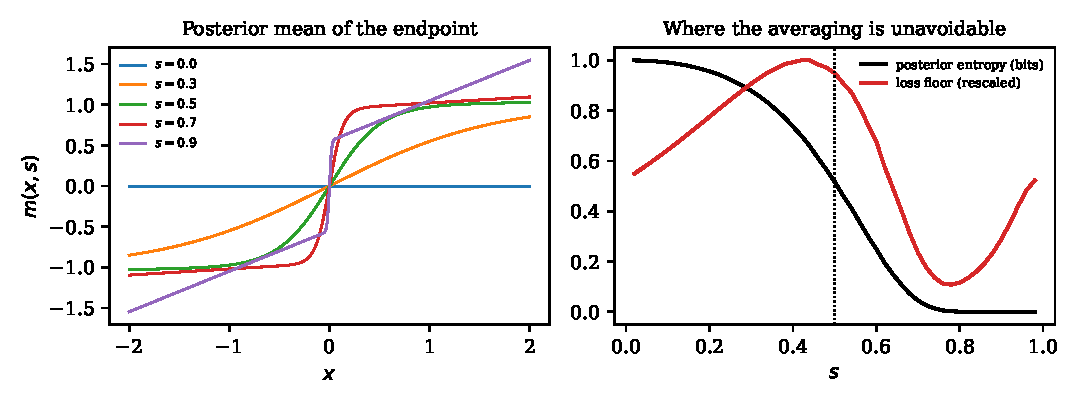
\includegraphics[width=\textwidth]{fig_field.pdf}
\caption{Left: the posterior mean $m(x,s)$ at five times. At $s=0$ it is the constant $0$, and it develops two plateaus near $\pm a$ as $s$ grows. Right: mean posterior entropy of the mode (bits) and the training-loss floor $L^\ast(s)$ rescaled to its maximum. The dotted line is $s_c$ (Section~4.2).}
\end{figure}

\section{The integrator is another average}

The exact field is not what a sampler uses. It uses Euler steps of finite size, and each step is itself a partial move toward a posterior mean.

\begin{proposition}
Suppose an Euler step of size $\Delta$ is taken from time $s$ with $\lambda=\Delta/(1-s)\le1$. The new position is
\[
x+\Delta\,v^\ast(x,s)=(1-\lambda)\,x+\lambda\,m(x,s).
\]
In particular, on the last step of a uniform schedule, $\Delta=1-s$, so $\lambda=1$ and the output is exactly $m(x,1-\Delta)$.
\end{proposition}

\begin{proof}
Substitute $v^\ast=(m-x)/(1-s)$. \qedhere
\end{proof}

Whatever the quality of the earlier steps, the final sample is the posterior mean of the endpoint given the penultimate position. Within a mode this is a shrunken version of the data. Take the penultimate position drawn from its true marginal at $s=1-\Delta$. As a within-mode approximation, valid when the mode is identified with high probability, the within-component part of the output has standard deviation
\[
\frac{s\sigma^2}{\tau(s)}=\sigma\cdot\frac{s\sigma}{\tau(s)}=\sigma\Big/\sqrt{1+\dfrac{(1-s)^2}{s^2\sigma^2}}\ \approx\ \sigma\Big/\sqrt{1+(\Delta/\sigma)^2}.
\]
The ratio of output spread to data spread is therefore a function of $\Delta/\sigma$ alone. When $\Delta\ll\sigma$ the ratio tends to one and the last step is harmless. When $\Delta\gtrsim\sigma$ the output collapses within each mode toward its center, and when $\Delta$ is comparable to $a$ the posterior weights are no longer decisive and the output moves toward the global mean. The final step reintroduces endpoint averaging at the scale of the final step.

For a $K$-step uniform schedule the final step size is $1/K$, so the last step alone is faithful at the within-mode scale when $K\gg1/\sigma$ and at the between-mode scale when $K\gg1/a$. The formula is evaluated on the true penultimate marginal. In a full sampler the penultimate distribution is itself affected by earlier Euler errors, so the observed spread need not match it.

\section{Simulation}

The simulation uses $a=1$, $\sigma=0.1$, and $N=2\times10^5$ source samples integrated with $K$ uniform Euler steps under the exact field. Table~1 is a single seeded run. The reference is an independent sample of $N$ target points. Table~1 reports, for each $K$, the fraction of outputs in the gap $|x|<a/2$, the within-sign standard deviation relative to $\sigma$, and the 1-Wasserstein distance to the reference.

\begin{table}[t]
\centering
\caption{Euler integration of the exact field, $a=1$, $\sigma=0.1$. Within-sign spread is the average standard deviation of the positive and negative output groups divided by $\sigma$; it is undefined at $K=1$ because every output equals $0$. Across six independent seeds at $K=2048$ the Wasserstein distance between two independent samples ranges from $0.002$ to $0.006$ (mean $0.0037$), so values below about $5\times10^{-3}$, those for $K\ge64$, are not resolved at this sample size.}
\begin{tabular}{rcccc}
\toprule
$K$ & gap mass & within-sign spread$/\sigma$ & $W_1$ to target \\
\midrule
1    & 1.000   & undefined & 1.000 \\
2    & 0.421   & 2.94 & 0.445 \\
3    & 0.134   & 2.59 & 0.168 \\
4    & 0.0487  & 1.75 & 0.0768 \\
8    & 0.0020  & 0.82 & 0.0295 \\
16   & 0.00029 & 0.87 & 0.0160 \\
32   & 0.00003 & 0.93 & 0.0086 \\
64   & 0.000005 & 0.96 & 0.0046 \\
256  & 0 & 0.99 & 0.0015 \\
2048 & 0 & 1.00 & 0.0007 \\
\bottomrule
\end{tabular}
\end{table}

Three features of the table matter. First, $K=1$ reproduces Proposition~1: all mass sits at $0$. Second, the gap mass falls quickly. In this run, about $0.2\%$ of the output lies between the modes at $K=8$, so the bimodality is recovered at a very coarse resolution. The decrease with $K$ is an observation at the tested step counts, not a monotonicity theorem. Third, the spread is not monotone in $K$. For $K\le4$ it is inflated, because the sign split mixes outputs that have not yet committed. For $K=8$ it falls to $0.82\sigma$, then climbs back toward $\sigma$ as $K$ grows. The dip is consistent with the last-step shrinkage of Section~5, though not explained by it alone, as the next comparison shows.

To isolate the last-step mechanism the simulation also draws the penultimate position from its true marginal and applies the last step. Table~2 compares the observed within-mode spread ratio, from a single seed, with the prediction $s\sigma/\tau(s)$ at $s=1-\Delta$. The prediction assumes identified modes and applies for $\Delta\le1/8$ in this parameter setting. At larger $\Delta$ the posterior weights are not decisive and the within-sign spread is inflated by mode mixing instead; the observed ratios at $\Delta=1/2$ and $1/4$ are $2.95$ and $0.53$, against predictions of $0.10$ and $0.29$, and are reported here only to mark where the formula stops applying.

\begin{table}[t]
\centering
\caption{Last step from the true marginal at $s=1-\Delta$. Ratio of within-mode output spread to $\sigma$, observed and predicted by $s\sigma/\tau(s)$.}
\begin{tabular}{rcc}
\toprule
$\Delta$ & observed & predicted \\
\midrule
$1/8$   & 0.573 & 0.573 \\
$1/16$  & 0.833 & 0.832 \\
$1/32$  & 0.954 & 0.952 \\
$1/64$  & 0.989 & 0.988 \\
$1/256$ & 0.9995 & 0.9992 \\
\bottomrule
\end{tabular}
\end{table}

Over six independent seeds the mean ratios agree with the prediction to within $0.0005$, with a standard deviation across seeds of $0.0014$ to $0.0022$, so the agreement is within about $0.002$ in spread ratio. This verifies the last-step shrinkage mechanism. It does not show that the full sampler's spread is explained by it. At $K=8$ the full sampler's ratio is $0.82$ against $0.57$ for the isolated last step, and at $K=16$ it is $0.87$ against $0.83$. The full sampler additionally reflects accumulated integration error, which can offset or amplify the shrinkage.

\begin{figure}[t]
\centering
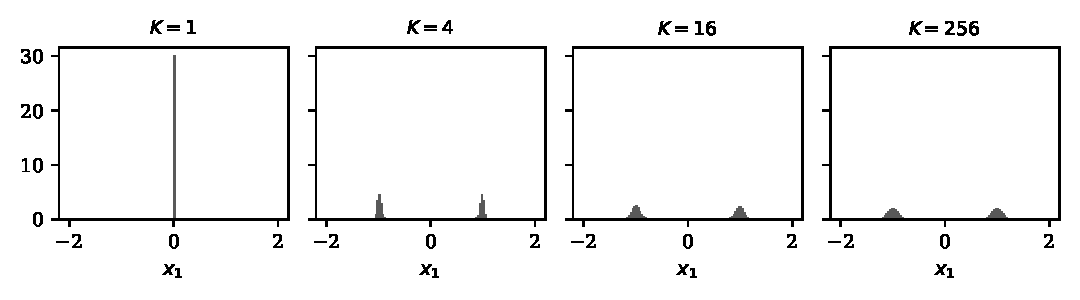
\includegraphics[width=\textwidth]{fig_euler.pdf}
\caption{Output histograms from the exact field with $K=1,4,16,256$ Euler steps. $K=1$ is a point mass at the mean.}
\end{figure}

\section{Application to a multi-anchor exploration paper}

A recent paper on active three-dimensional mapping argues that regressing a single next-best view averages incompatible directions and that a flow-matching proposal model avoids this \citep{li2026}. The derivation above bears on that argument in three ways, each stated within what the model licenses.

First, the claim ``flow matching avoids averaging'' holds for the exact field integrated finely. It does not hold for a one-step sampler, which is the regression mean by Proposition~1. A system that reports results as a function of the number of integration steps is therefore reporting, in part, how far it is from the regression solution. Whether the final step of a given schedule is small relative to the spread of anchors within a mode depends on the units in which the anchors are expressed, and Section~5 shows that this ratio is the controlling quantity. The paper does not report it, so the analysis cannot say on which side of the threshold that system sits.

Second, the paper's anchors are structured vectors, not scalars, and its orientation components live on a circle. The two-mode analysis does not transfer to those components without work, and the analysis does not show that the problem the paper addresses is of the two-mode kind. It shows what would be true if it were. Likewise, nothing here shows that a particular system's proposal distribution is limited by its integrator.

Third, nothing in the analysis addresses whether proposals are \emph{useful}. A sampler can reproduce the proposal distribution exactly and still be paired with a selector that cannot tell which proposals are worth following. Averaging of endpoints and quality of selection are separate matters, and the benefit attributed to avoiding the former has to be established separately from the benefit of the latter.

\section{Four misreadings}

\paragraph{``Regression averages and generation does not.''} Both average. The regressor averages endpoints given the observation. The flow averages velocities given observation, position and time. The statement that survives is about what is averaged and what the average is conditioned on, and about how those change along the path.

\paragraph{``Straight paths mean the model drives samples toward the mean.''} The conditional paths are straight and cross. The marginal field is their average, and the integral curves of the average are separated by construction. The mean enters only when the integrator is too coarse to follow the field through the interval around $s_c$.

\paragraph{``A flow model is generative whatever the number of steps.''} A one-step flow with the exact field is the regression solution (Proposition~1). Calling a model generative describes the sampler and the field together, not the loss.

\paragraph{``More steps always fix it.''} For the exact field, the gap mass and Wasserstein distance decreased with $K$ at the step counts tested. A learned field has an error that need not decrease with $K$, and Table~1 is an exact-field reference calculation, not a lower bound for networks: a learned field can differ from the exact one in ways that compensate for a coarse integrator. The large local gradients near the end of the path suggest that errors in a learned field could matter there, but that is a hypothesis to test, not a result.

\section{Limits}

The analysis is one-dimensional with two symmetric Gaussian components. It uses the exact field. Real systems use a network that approximates a field in many dimensions, with correlated components and unequal weights, and the closed forms here do not apply to them. The scale $\sigma$ is the within-mode spread in whatever units the data are expressed in, and a system's behavior depends on the ratio of its last step to that spread. That ratio is not the same across parameterizations, and comparisons of step counts across systems that use different units are not comparisons of the same quantity. Finally, the simulation validates the formulas, which are exact in the model. It does not validate the model as a description of any particular dataset.

\appendix
\section{Derivations}

\paragraph{Posterior mean.} Given component $k$, $(x_1,x_s)$ is jointly Gaussian with $\Var(x_1)=\sigma^2$, $\operatorname{Cov}(x_1,x_s)=s\sigma^2$ and $\Var(x_s)=\tau^2$. The conditional mean is $\mu_k+(s\sigma^2/\tau^2)(x-s\mu_k)$ and the conditional variance is $\sigma^2-s^2\sigma^4/\tau^2=\sigma^2(1-s)^2/\tau^2$, using $\tau^2-s^2\sigma^2=(1-s)^2$.

\paragraph{Weights.} $w_k\propto\pi_k\exp\{-(x-s\mu_k)^2/2\tau^2\}$. The ratio $w_+/w_-=\exp\{(2as\,x)/\tau^2\}$ because the quadratic terms in $x$ cancel.

\paragraph{Total posterior variance.} $\Var(x_1\mid x_s)=\sum_k w_k\big[\sigma^2(1-s)^2/\tau^2+(m_k-m)^2\big]$, by the law of total variance within the mixture posterior.

\paragraph{Bayes error.} Given $k=+$, $x_s\sim\N(sa,\tau^2)$, and given $k=-$, $x_s\sim\N(-sa,\tau^2)$. The likelihood-ratio test with equal priors thresholds at $0$ and errs with probability $\Phi(-sa/\tau)$. The log-odds at $x_s=sa+\tau z$ is $2as(sa+\tau z)/\tau^2=2d^2+2dz$, which has mean $2d^2$ and variance $4d^2$.

\paragraph{Jacobian at the midpoint.} At $x=0$, $w_\pm=\tfrac12$, $m_\pm(0)=\pm a(1-s)^2/\tau^2$ and $\partial_xw_+=as/(2\tau^2)$. Then $\partial_xm=s\sigma^2/\tau^2+a^2s(1-s)^2/\tau^4$ and $\partial_xv^\ast=(\partial_xm-1)/(1-s)$. With $s\approx1$ the second term dominates and equals $a^2u/(\sigma^2+u^2)^2$ for $u=1-s$, maximized at $u=\sigma/\sqrt3$ with value $9a^2/(16\sqrt3\,\sigma^3)\approx0.325\,a^2/\sigma^3$. The exact maximum for $a=1,\sigma=0.1$ is $360.9$ at $s=0.942$, so the approximation underestimates it by about ten percent.

\paragraph{Last-step spread.} Given component $+$, the within-component part of $m(x_s,s)$ is $\mu_++(s\sigma^2/\tau^2)(x_s-s\mu_+)$ when $w_+\approx1$. Since $x_s-s\mu_+\sim\N(0,\tau^2)$, this has standard deviation $s\sigma^2/\tau$, and the ratio to $\sigma$ is $s\sigma/\tau$.

\section{Simulation details}

Source samples are drawn from $\N(0,1)$ with a fixed seed. The exact field is evaluated by the closed forms above, with the logistic weights computed in log space. Euler steps are uniform on $[0,1]$ with the last step ending at $s=1$ and the field evaluated only at $s<1$. Within-sign spread splits outputs by sign and averages the two standard deviations. The Wasserstein distance is the mean absolute difference between sorted samples. Posterior entropy and the loss floor are estimated from $4\times10^4$ draws of $(x_1,x_s)$ at each of 49 times in $[0.02,0.98]$. The script \texttt{sim.py} and the numerical outputs accompany the essay. The repeated-seed checks use six seeds in \texttt{seeds.py}.

\begin{thebibliography}{9}
\bibitem[Lipman et al.(2023)]{lipman2023}
Y.~Lipman, R.~T.~Q. Chen, H.~Ben-Hamu, M.~Nickel and M.~Le.
\newblock Flow matching for generative modeling.
\newblock \emph{International Conference on Learning Representations}, 2023. arXiv:2210.02747.

\bibitem[Li et al.(2026)]{li2026}
Y.~Li, A.~Wu, Z.~Zhang, Z.~Han, S.~Zhang and Y.~Han.
\newblock All roads lead to Rome: flow-driven multi-anchor exploration for open-environment active 3D mapping.
\newblock arXiv:2609.36889, 2026.
\end{thebibliography}

\end{document}
